%Chapter 1
\chapter{Introduction and background}  %J.H Marais, C.J.R. Kriel
\pagenumbering{arabic}
\thispagestyle{empty}
\vspace{38em}
\hrulefill
\\
\enquote*{\textit{Quote.}} - Somebody\\
\newpage

\section{Preamble}
This chapter firstly discusses background regarding deep level mining in South Africa. Next, the need to reduce costs of operation in the mining sector is examined. From this a focus in reducing energy consumption of compressed air systems is developed. Next, background on compressed air operation and energy interventions are discussed. Simulations and their value in industry is discussed leading to a problem statement and objectives of the study. Finally, an overview for the dissertation is provided.
\section{Background on deep level mining}
	\subsection{Mining profitability}
	\footnotetext[1]{inflation.eu, "Historic inflation South Africa." [Online] \url{http://www.inflation.eu/inflation-rates/south-africa/historic-inflation/cpi-inflation-south-africa.aspx}, [Accessed 25 March 2017].}
	 	Various technical, economic, social and operational challenges are posing a risk to the profitability of the South African mining sector. One of the challenges the sector faces  is a rise in the cost of operation \cite{neingo2016trends}.
	 	\par
		A considerable factor that is contributing to the rise of operational costs in South African gold mines has been the increase in electricity costs. As shown in \cref{fig: Eskom tariffs}, the general cost of electricity has increased at a rate greater than inflation since 2008 \cite{Eskom2013Tariffs}.
		\begin{figure}[h]
			\centering
			\fbox{% GNUPLOT: LaTeX picture with Postscript
\begingroup
  \makeatletter
  \providecommand\color[2][]{%
    \GenericError{(gnuplot) \space\space\space\@spaces}{%
      Package color not loaded in conjunction with
      terminal option `colourtext'%
    }{See the gnuplot documentation for explanation.%
    }{Either use 'blacktext' in gnuplot or load the package
      color.sty in LaTeX.}%
    \renewcommand\color[2][]{}%
  }%
  \providecommand\includegraphics[2][]{%
    \GenericError{(gnuplot) \space\space\space\@spaces}{%
      Package graphicx or graphics not loaded%
    }{See the gnuplot documentation for explanation.%
    }{The gnuplot epslatex terminal needs graphicx.sty or graphics.sty.}%
    \renewcommand\includegraphics[2][]{}%
  }%
  \providecommand\rotatebox[2]{#2}%
  \@ifundefined{ifGPcolor}{%
    \newif\ifGPcolor
    \GPcolortrue
  }{}%
  \@ifundefined{ifGPblacktext}{%
    \newif\ifGPblacktext
    \GPblacktextfalse
  }{}%
  % define a \g@addto@macro without @ in the name:
  \let\gplgaddtomacro\g@addto@macro
  % define empty templates for all commands taking text:
  \gdef\gplbacktext{}%
  \gdef\gplfronttext{}%
  \makeatother
  \ifGPblacktext
    % no textcolor at all
    \def\colorrgb#1{}%
    \def\colorgray#1{}%
  \else
    % gray or color?
    \ifGPcolor
      \def\colorrgb#1{\color[rgb]{#1}}%
      \def\colorgray#1{\color[gray]{#1}}%
      \expandafter\def\csname LTw\endcsname{\color{white}}%
      \expandafter\def\csname LTb\endcsname{\color{black}}%
      \expandafter\def\csname LTa\endcsname{\color{black}}%
      \expandafter\def\csname LT0\endcsname{\color[rgb]{1,0,0}}%
      \expandafter\def\csname LT1\endcsname{\color[rgb]{0,1,0}}%
      \expandafter\def\csname LT2\endcsname{\color[rgb]{0,0,1}}%
      \expandafter\def\csname LT3\endcsname{\color[rgb]{1,0,1}}%
      \expandafter\def\csname LT4\endcsname{\color[rgb]{0,1,1}}%
      \expandafter\def\csname LT5\endcsname{\color[rgb]{1,1,0}}%
      \expandafter\def\csname LT6\endcsname{\color[rgb]{0,0,0}}%
      \expandafter\def\csname LT7\endcsname{\color[rgb]{1,0.3,0}}%
      \expandafter\def\csname LT8\endcsname{\color[rgb]{0.5,0.5,0.5}}%
    \else
      % gray
      \def\colorrgb#1{\color{black}}%
      \def\colorgray#1{\color[gray]{#1}}%
      \expandafter\def\csname LTw\endcsname{\color{white}}%
      \expandafter\def\csname LTb\endcsname{\color{black}}%
      \expandafter\def\csname LTa\endcsname{\color{black}}%
      \expandafter\def\csname LT0\endcsname{\color{black}}%
      \expandafter\def\csname LT1\endcsname{\color{black}}%
      \expandafter\def\csname LT2\endcsname{\color{black}}%
      \expandafter\def\csname LT3\endcsname{\color{black}}%
      \expandafter\def\csname LT4\endcsname{\color{black}}%
      \expandafter\def\csname LT5\endcsname{\color{black}}%
      \expandafter\def\csname LT6\endcsname{\color{black}}%
      \expandafter\def\csname LT7\endcsname{\color{black}}%
      \expandafter\def\csname LT8\endcsname{\color{black}}%
    \fi
  \fi
    \setlength{\unitlength}{0.0500bp}%
    \ifx\gptboxheight\undefined%
      \newlength{\gptboxheight}%
      \newlength{\gptboxwidth}%
      \newsavebox{\gptboxtext}%
    \fi%
    \setlength{\fboxrule}{0.5pt}%
    \setlength{\fboxsep}{1pt}%
\begin{picture}(9360.00,4032.00)%
    \gplgaddtomacro\gplbacktext{%
      \colorrgb{0.00,0.00,0.00}%
      \put(682,1144){\makebox(0,0)[r]{\strut{}$0$}}%
      \colorrgb{0.00,0.00,0.00}%
      \put(682,1422){\makebox(0,0)[r]{\strut{}$5$}}%
      \colorrgb{0.00,0.00,0.00}%
      \put(682,1701){\makebox(0,0)[r]{\strut{}$10$}}%
      \colorrgb{0.00,0.00,0.00}%
      \put(682,1979){\makebox(0,0)[r]{\strut{}$15$}}%
      \colorrgb{0.00,0.00,0.00}%
      \put(682,2258){\makebox(0,0)[r]{\strut{}$20$}}%
      \colorrgb{0.00,0.00,0.00}%
      \put(682,2536){\makebox(0,0)[r]{\strut{}$25$}}%
      \colorrgb{0.00,0.00,0.00}%
      \put(682,2814){\makebox(0,0)[r]{\strut{}$30$}}%
      \colorrgb{0.00,0.00,0.00}%
      \put(682,3093){\makebox(0,0)[r]{\strut{}$35$}}%
      \colorrgb{0.00,0.00,0.00}%
      \put(682,3371){\makebox(0,0)[r]{\strut{}$40$}}%
      \colorrgb{0.00,0.00,0.00}%
      \put(814,924){\makebox(0,0){\strut{}$2006$}}%
      \colorrgb{0.00,0.00,0.00}%
      \put(2172,924){\makebox(0,0){\strut{}$2008$}}%
      \colorrgb{0.00,0.00,0.00}%
      \put(3530,924){\makebox(0,0){\strut{}$2010$}}%
      \colorrgb{0.00,0.00,0.00}%
      \put(4888,924){\makebox(0,0){\strut{}$2012$}}%
      \colorrgb{0.00,0.00,0.00}%
      \put(6246,924){\makebox(0,0){\strut{}$2014$}}%
      \colorrgb{0.00,0.00,0.00}%
      \put(7604,924){\makebox(0,0){\strut{}$2016$}}%
      \colorrgb{0.00,0.00,0.00}%
      \put(8962,924){\makebox(0,0){\strut{}$2018$}}%
    }%
    \gplgaddtomacro\gplfronttext{%
      \csname LTb\endcsname%
      \put(176,2257){\rotatebox{-270}{\makebox(0,0){\strut{}\% increase}}}%
      \put(4888,594){\makebox(0,0){\strut{}Year}}%
      \put(4888,3701){\makebox(0,0){\strut{}Electricity price increases in South Africa}}%
      \csname LTb\endcsname%
      \put(6770,393){\makebox(0,0)[r]{\strut{}Eskom general tariff increases (\%)}}%
      \csname LTb\endcsname%
      \put(1493,1562){\makebox(0,0){\strut{}6.0}}%
      \put(2172,2759){\makebox(0,0){\strut{}27.5}}%
      \put(2851,2970){\makebox(0,0){\strut{}31.3}}%
      \put(3530,2608){\makebox(0,0){\strut{}24.8}}%
      \put(4209,2664){\makebox(0,0){\strut{}25.8}}%
      \put(4888,2118){\makebox(0,0){\strut{}16.0}}%
      \put(5567,1673){\makebox(0,0){\strut{}8.0}}%
      \put(6246,1673){\makebox(0,0){\strut{}8.0}}%
      \put(6925,1673){\makebox(0,0){\strut{}8.0}}%
      \put(7604,1673){\makebox(0,0){\strut{}8.0}}%
      \put(8283,1673){\makebox(0,0){\strut{}8.0}}%
      \csname LTb\endcsname%
      \put(6770,173){\makebox(0,0)[r]{\strut{}Inflation rate in south Africa (\%)}}%
    }%
    \gplbacktext
    \put(0,0){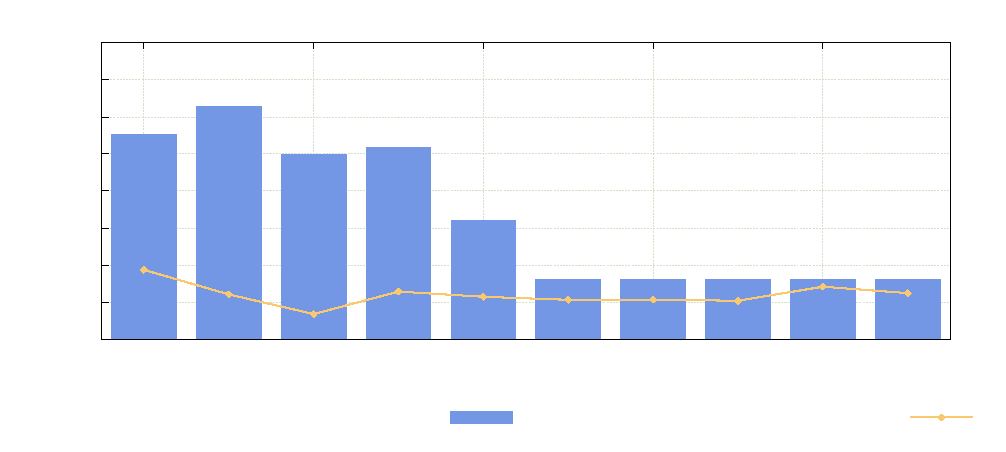
\includegraphics{Graphs/1/Eskom/Eskom}}%
    \gplfronttext
  \end{picture}%
\endgroup
}
			\caption[Electricity price increases between 2007 and 2017 compared to the inflation rate in South Africa..]{Electricity price increases between 2007 and 2017 \cite{Eskom2013Tariffs} compared to the inflation rate in South Africa\protect\footnotemark[1]. }
			\label{fig: Eskom tariffs}
		\end{figure}
		\par
		In addition to rising electricity costs, gold ore grades of South African mines have fallen substantially over the last few decades \cite{mudd2007global}. As ore grades decline, the energy utilised per unit of metal increases exponentially \cite{muller2010numerical}. Therefore mines require significantly more energy per unit of metal produced. This combination of tariff increases and increased energy usage per unit have led to significant rises in mining operation costs.
	\subsection{Process of a deep level mine}
	South Africa's mines are some of the deepest in the world Some mine shafts are reaching depths deeper than $4000m$ below the surface \cite{vosloo2012case}. The process of extracting ore at this depth is dependent on the essential services, mainly cooling and ventilation, pumping, compressed air and hoisting, as shown in \cref{fig: Mining Layout}.
	\par 
	 Cooling and ventilation system are required to maintain a safe working temperature underground. Pumping is critical to remove service and fissure water, preventing flooding. Compressed air is needed to safely power underground drills and machines. Finally, hoisting systems are used to bring the ore to the surface and to transport mine workers in the mine. 
		\begin{figure}[h!]
			\centering
			\fbox{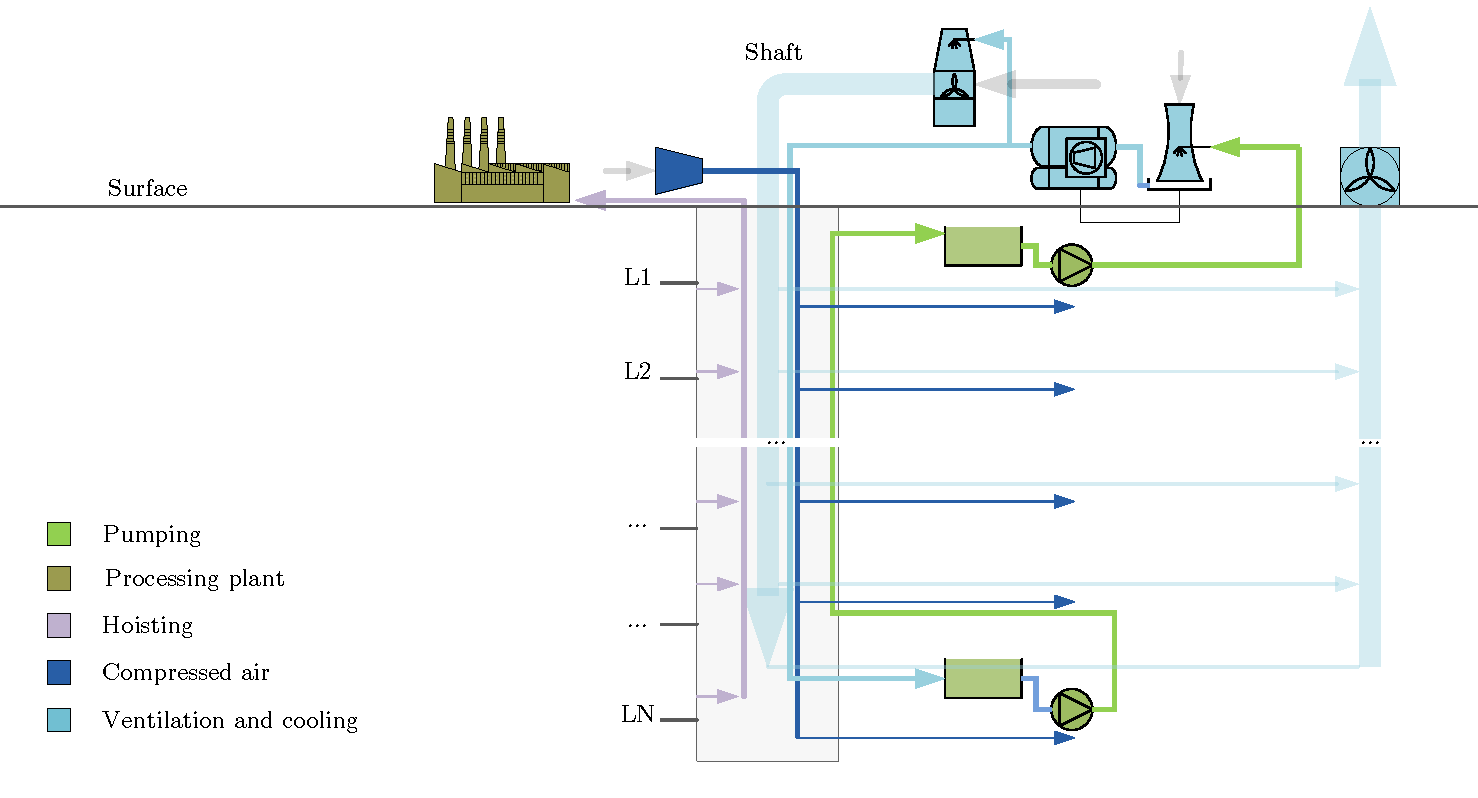
\includegraphics[width=\textwidth]{Graphs/1/Layout/Layout.pdf}}
			\caption{A layout showing the mining processes.}
			\label{fig: Mining Layout}
		\end{figure}
		\subsubsection{Energy usage of mining services}
			The mining industry uses extensive amounts of energy. In South Africa, the industry utilizes approximately 15\% of the national electricity supplier's yearly output, of which, gold and platinum mines use 80\%.\cite{Eskom2010Energy}
			\par
			 \cref{fig: Energy Split} shows the division of energy within the mining industry. The chart shows that compressed air systems utilizes the most energy within a mining industry. It is reasoned that energy can be most effectively reduced through the implementation of energy interventions on compressed air systems.
			\begin{figure}[h]
				\centering
				\fbox{% GNUPLOT: LaTeX picture with Postscript
\begingroup
  \makeatletter
  \providecommand\color[2][]{%
    \GenericError{(gnuplot) \space\space\space\@spaces}{%
      Package color not loaded in conjunction with
      terminal option `colourtext'%
    }{See the gnuplot documentation for explanation.%
    }{Either use 'blacktext' in gnuplot or load the package
      color.sty in LaTeX.}%
    \renewcommand\color[2][]{}%
  }%
  \providecommand\includegraphics[2][]{%
    \GenericError{(gnuplot) \space\space\space\@spaces}{%
      Package graphicx or graphics not loaded%
    }{See the gnuplot documentation for explanation.%
    }{The gnuplot epslatex terminal needs graphicx.sty or graphics.sty.}%
    \renewcommand\includegraphics[2][]{}%
  }%
  \providecommand\rotatebox[2]{#2}%
  \@ifundefined{ifGPcolor}{%
    \newif\ifGPcolor
    \GPcolortrue
  }{}%
  \@ifundefined{ifGPblacktext}{%
    \newif\ifGPblacktext
    \GPblacktextfalse
  }{}%
  % define a \g@addto@macro without @ in the name:
  \let\gplgaddtomacro\g@addto@macro
  % define empty templates for all commands taking text:
  \gdef\gplbacktext{}%
  \gdef\gplfronttext{}%
  \makeatother
  \ifGPblacktext
    % no textcolor at all
    \def\colorrgb#1{}%
    \def\colorgray#1{}%
  \else
    % gray or color?
    \ifGPcolor
      \def\colorrgb#1{\color[rgb]{#1}}%
      \def\colorgray#1{\color[gray]{#1}}%
      \expandafter\def\csname LTw\endcsname{\color{white}}%
      \expandafter\def\csname LTb\endcsname{\color{black}}%
      \expandafter\def\csname LTa\endcsname{\color{black}}%
      \expandafter\def\csname LT0\endcsname{\color[rgb]{1,0,0}}%
      \expandafter\def\csname LT1\endcsname{\color[rgb]{0,1,0}}%
      \expandafter\def\csname LT2\endcsname{\color[rgb]{0,0,1}}%
      \expandafter\def\csname LT3\endcsname{\color[rgb]{1,0,1}}%
      \expandafter\def\csname LT4\endcsname{\color[rgb]{0,1,1}}%
      \expandafter\def\csname LT5\endcsname{\color[rgb]{1,1,0}}%
      \expandafter\def\csname LT6\endcsname{\color[rgb]{0,0,0}}%
      \expandafter\def\csname LT7\endcsname{\color[rgb]{1,0.3,0}}%
      \expandafter\def\csname LT8\endcsname{\color[rgb]{0.5,0.5,0.5}}%
    \else
      % gray
      \def\colorrgb#1{\color{black}}%
      \def\colorgray#1{\color[gray]{#1}}%
      \expandafter\def\csname LTw\endcsname{\color{white}}%
      \expandafter\def\csname LTb\endcsname{\color{black}}%
      \expandafter\def\csname LTa\endcsname{\color{black}}%
      \expandafter\def\csname LT0\endcsname{\color{black}}%
      \expandafter\def\csname LT1\endcsname{\color{black}}%
      \expandafter\def\csname LT2\endcsname{\color{black}}%
      \expandafter\def\csname LT3\endcsname{\color{black}}%
      \expandafter\def\csname LT4\endcsname{\color{black}}%
      \expandafter\def\csname LT5\endcsname{\color{black}}%
      \expandafter\def\csname LT6\endcsname{\color{black}}%
      \expandafter\def\csname LT7\endcsname{\color{black}}%
      \expandafter\def\csname LT8\endcsname{\color{black}}%
    \fi
  \fi
    \setlength{\unitlength}{0.0500bp}%
    \ifx\gptboxheight\undefined%
      \newlength{\gptboxheight}%
      \newlength{\gptboxwidth}%
      \newsavebox{\gptboxtext}%
    \fi%
    \setlength{\fboxrule}{0.5pt}%
    \setlength{\fboxsep}{1pt}%
\begin{picture}(9360.00,3528.00)%
    \gplgaddtomacro\gplbacktext{%
      \colorrgb{0.00,0.00,0.00}%
      \put(682,440){\makebox(0,0)[r]{\strut{}$0$}}%
      \colorrgb{0.00,0.00,0.00}%
      \put(682,1005){\makebox(0,0)[r]{\strut{}$5$}}%
      \colorrgb{0.00,0.00,0.00}%
      \put(682,1569){\makebox(0,0)[r]{\strut{}$10$}}%
      \colorrgb{0.00,0.00,0.00}%
      \put(682,2134){\makebox(0,0)[r]{\strut{}$15$}}%
      \colorrgb{0.00,0.00,0.00}%
      \put(682,2698){\makebox(0,0)[r]{\strut{}$20$}}%
      \colorrgb{0.00,0.00,0.00}%
      \put(682,3263){\makebox(0,0)[r]{\strut{}$25$}}%
      \colorrgb{0.00,0.00,0.00}%
      \put(1323,150){\makebox(0,0){\strut{}\scriptsize{\shortstack{Compressed \\ air}}}}%
      \colorrgb{0.00,0.00,0.00}%
      \put(2342,150){\makebox(0,0){\strut{}\scriptsize{\shortstack{Mining \\ processes}}}}%
      \colorrgb{0.00,0.00,0.00}%
      \put(3360,150){\makebox(0,0){\strut{}\scriptsize{\shortstack{Pumping}}}}%
      \colorrgb{0.00,0.00,0.00}%
      \put(4379,150){\makebox(0,0){\strut{}\scriptsize{\shortstack{Ventilation \\ and cooling}}}}%
      \colorrgb{0.00,0.00,0.00}%
      \put(5397,150){\makebox(0,0){\strut{}\scriptsize{\shortstack{Buildings \\ and hostels}}}}%
      \colorrgb{0.00,0.00,0.00}%
      \put(6416,150){\makebox(0,0){\strut{}\scriptsize{\shortstack{Processing \\ plant}}}}%
      \colorrgb{0.00,0.00,0.00}%
      \put(7434,150){\makebox(0,0){\strut{}\scriptsize{\shortstack{Hoisting}}}}%
      \colorrgb{0.00,0.00,0.00}%
      \put(8453,150){\makebox(0,0){\strut{}\scriptsize{\shortstack{Other}}}}%
    }%
    \gplgaddtomacro\gplfronttext{%
      \csname LTb\endcsname%
      \put(176,1851){\rotatebox{-270}{\makebox(0,0){\strut{}\% of total energy consumption}}}%
    }%
    \gplbacktext
    \put(0,0){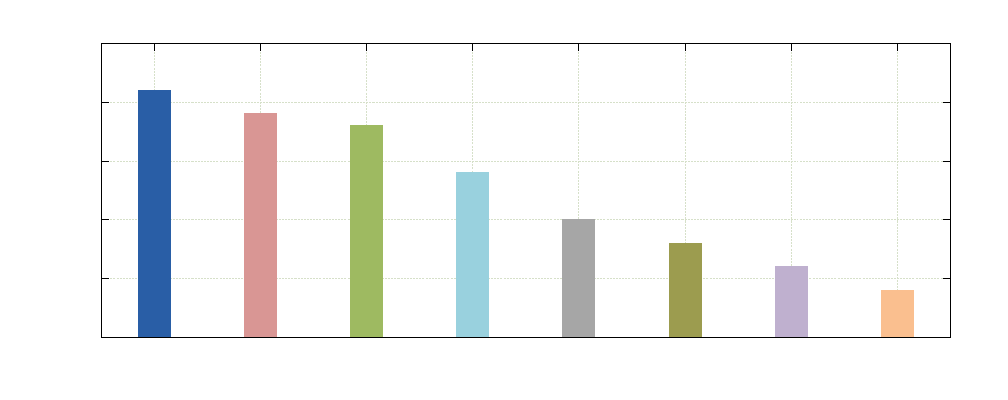
\includegraphics{Graphs/1/distribution/distribution}}%
    \gplfronttext
  \end{picture}%
\endgroup
}
				\caption[The energy consumption for each mining system.]{The energy consumption for each mining system \cite{le2005energy}.}
				\label{fig: Energy Split}
			\end{figure}
\section{Compressed air systems in mining}
	\subsection{Compressed air in operation}\label{key}
		Largely due to their reliability, versatilely and ease of use, the South African mining industry has installed extensive compressed air networks. These systems can have compressors with capacities of up to 15 Mega\gls*{w} ($MW$) \cite{Marais2012PhD}.
		However, the supply of compressed air is a highly energy demanding and costly process \cite{padachi2009energy}.  The energy used for compressed air production contributes to between 9\% and 20\% of the total mining energy consumption	\cite{Eskom2010Energy},\cite{du2011development}. 
		\par
		Large compressed air systems are likely inefficient. Internationally, the expected energy savings potential of a large compressed air network is 15\% \cite{neale2009compressed}. Marais \cite{marais2013simplification} showed that energy saving interventions can lead to energy and cost savings of up to 30\% and 40\%. 
	 
	\subsection{Characteristic inefficiencies of compressed air systems}
		Compressed air distribution networks in the mining industry consist of multiple compressors and working areas up to eight kilometres away from the source \cite{Marais2012PhD}. Due to their size and complexity, these systems are prone to large energy losses.
		\par 
		Compressed air leakage accounts for as much as 35\% of the energy losses of a compressed air network \cite{Lawrence2004Improving}. Other systemic losses include, faulty valves, pipe diameter fluctuations, obstructed air compressor intake filters and inefficient compressors. 	
	
		Leakage and inefficiency detection strategies are not often pursued in the South African mining industry \cite{vanTonder2010Masters}. Many mines do however perform leak inspections either internally or by a outside company. In these inspections, an ultrasonic detector is used to locate the leak. Alternatively, some mines employ the \enquote{walk and listen} method to identify leaks from the audible sound that it produces \cite{vanTonder2010Masters}. Once the inspection is completed, the findings, including the locations and estimated costs of all identified leaks, are reported.
		
	\subsection{Compressed air savings interventions}
		Energy interventions to reduce energy on compressed air systems designed using the following strategies \cite{Snyman2011Masters}:
		\begin{itemize}
			\item Reduce leaks.
			\item Reduce demand.
			\item Reduce unauthorised usage.
			\item Increase supply efficiency.
			\item Optimise supply.
		\end{itemize}
	 Often a combination of energy strategies will lead to the most savings \cite{Marais2012PhD}. In \cref{Chap2}, Successfully  compressed air interventions on mining systems we be discussed from literature.
	 \par 
	 Once a energy saving measure has been identified, it is most often necessary to make estimations to determine the potential costs and benefits of the intervention. This has usually been performed using first principle calculations, simplified mathematical models and practical tests if possible. However new tools have enabled quick, accurate compressed air model development. Through simulations, accurate estimations can be obtained quickly, with no risk and at comparatively low resource requirement.
\section{Use of simulation in industry }
	\subsection{Background in industrial simulation}
	
		Continuous improvements in computing hardware has led to major advancement in software technology. Consequently, the use of computational simulation has become an increasingly valuable tool for many industries.\cite{kocsis2003integration} \par 
		In \textit{ Handbook of simulation: principles, methodology, advances, applications, and practice}, the advantages of the use of simulation in industry are discussed as follows \cite{banks1998handbook}: 
		\begin{itemize}
			\item The ability to test new policies, operating procedures and methods without causing a disruption to the actual system.
			\item The means to identify problems in complex systems by gathering insight in the interactions within the system.
			\item The facility to compress or expand time to investigate phenomena thoroughly.
			\item The capability to determine the limits and constraints within a system.
			\item The potential to build consensus with regard to proposed designs or modifications.
		\end{itemize}

	\subsection{Simulation usage in compressed air optimisation}
		Simulation has been used to test and identify energy and operational improvements in mining compressed air systems. In the past producing complex models for mining systems was not feasible as simulation software required difficult to obtain data inputs \cite{marais2013simplification}. This lead to simplified models that cannot provide accurate results and limited the types of scenarios that can be simulated. 
		\par 
		However, the use of planned manual measurements, estimations  and new software technologies can overcome this challenge \cite{Bredenkamp2015Challeges},\cite{Mare2017Evaluating}. This would allow for the development of more detailed and accurate mining compressed air simulations.

\section{Problem statement and objectives}
	\subsection{Problem statement}
 		Rising costs and falling ore grades are driving the mining industry to reduce operational costs. The industry can save significant energy cost through interventions in compressed air systems. However, manual testing of these interventions are risky and cumbersome.
 		\par
 		Computer modelling and simulation of compressed air systems can be used to quantify and priorities operational interventions with minimal risk. However, simulations have not been utilised to their full potential in compressed air systems. With new tools and more detailed simulation models of mining systems the energy and operation efficiency of mining compressed air systems can be improved, leading to cost savings.3.
	\subsection{Research objectives}
		The main objective of this dissertation is to obtain energy savings through the identification of operational improvements in mining compressed air systems. A simulation process to will be developed to achieve this goal.
\section{Dissertation overview}
	\texttt{Describe (in approximately one sentence each) the contents of \\each of the dissertation chapters. No results here.}